\section{Motivation}

Satellite-derived data has become a key part of critical infrastructure for private, national, and scientific use.
Although new satellites are being launched at a high rate, even decades-old satellites are seeing novel use cases including advanced forest fire detection~\cite{nasaFirms} and analysis of activities in conflict areas~\cite{separatistLuminosity}. % TODO: cite a new forest fire paper, not FIRMS
These systems were built when robust cryptography was uncommon due to less powerful onboard computers.
It is now well accepted that legacy software which handles data without resilient authentication, such as these terrestrial processing systems, is not resilient against modern adversaries.
However, this was not a practical concern at the time since attacks at the physical layer would have required a costly and highly specialized setup.
Consequently, there does not exist any current work to understand the effects of a modern adversary against such a system.

Recent decades have seen a significant rise in the off-the-shelf availability of software-defined radio hardware, capable of emitting arbitrary signals at a wide range of frequencies.
This lowers the barrier to entry for signal injection attacks significantly.
Accordingly, both existing and novel use cases must now contend with the effects of signal injection, which include poisoning the dataset and exploiting the decoder.
This has far-reaching ramifications due to increased reliance on satellite-derived datasets.

\begin{figure}
    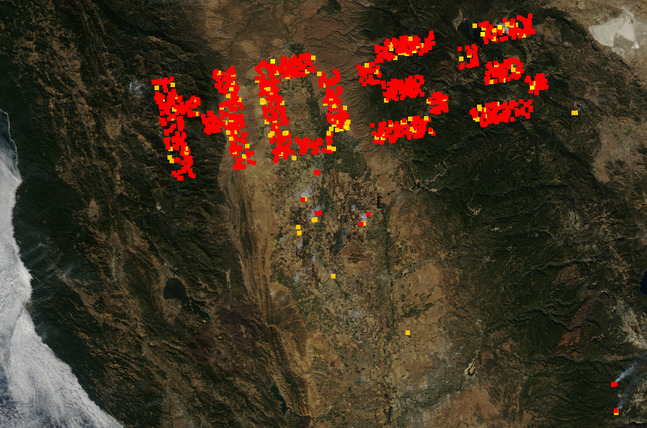
\includegraphics[width=\columnwidth]{diagrams/injection/pixels_800_140.jpg}
    \caption{An injected signal from the attacker manipulates the infrared channels of satellite imagery to create ficticious fires in the resulting dataset.}
    \label{fig:location-injection}
\end{figure}

As global reliance on this data increases, the security implications are becoming increasingly relevant.
Recent news demonstrates that motivated adversaries exist, and are interested in exploiting the decoding and demodulating pipelines.
For example, a recent attack against ViaSat's satellite broadband capabilities exploited side channel vulnerabilities in the terrestrial network, resulting in the receiver stations across Ukraine being permanently disabled; a move coinciding with the Russian invasion of the country~\cite{satcomAnalysis}.

To support a wide range of use cases, raw satellite data is processed into more specialized derived datasets such as for forest fire and storm detection.
This feeds into applications including critical national infrastructure and research-oriented purposes.
\textbf{TODO cite}
The importance of these applications makes attacking the raw data appealing.

Although these applications of satellite data are new, they rely on satellite infrastructure that was launched decades ago.
Since then radio hardware has become more accessible and knowledge of attacks on wireless systems has become more widespread.
Therefore, satellite-derived datasets and the processing systems that create them are now exposed to realistic attacks from far more adversaries -- in particular, data modification attacks from signal injection.
Critical services including NASA's \textit{Fire Information and Resource Management System} (FIRMS) can be affected (shown in Figure~\ref{fig:location-injection}) to trigger false emergency response or mislead crisis analysis.

The security community is becoming increasingly aware that radio overshadowing in a satellite context has the potential to affect critical services.
\textbf{TODO cite}
As a result, recent countermeasures have been proposed which analyze artifacts of overshadowing on the physical channel to determine the authenticity of the received data~\cite{jedermann2021orbit,oligeri2020past}.
However, the impact of signal overshadowing against currently-deployed satellites, and the real-world consequences on the systems that depend upon their data, have not yet been considered.

\subsection{Contributions}

Specifically, we make the following contributions:

\begin{itemize}
    \item We identify the capability of a modern adversary to affect satellite downlink processing systems using physical-layer attacks;
    \item We illustrate the problem using a full end-to-end case study against NASA's FIRMS service, demonstrating masking of forest fires and generation of fake fires. We further show denial of service and arbitrary code execution attacks on the processing systems themselves;
    \item We discuss the potential impact of similar attacks against other satellite-derived datasets, exploring the effects that an attacker could expect to cause in the real world;
    \item We analyze the feasibility of radio signal injection using commercial off-the-shelf equipment, taking into account the unique constraints of a terrestrial attacker against a highly directional dish;
    \item Finally, we examine the applicability of existing countermeasures, with respect to the unique constraints of this context.
\end{itemize}

    % TODO: something about categorising the attacks that are possible?

% Things to mention:
% * Recent satellite hacks, but none really focussing on the downlink system through radio
% * We require a systematisation to analyse the effects that an adversary could have
% * We need to show what real-world systems the attacker could expect to manipulate, so that we can secure them. To do this, we need to follow through a system end-to-end, and extract the general principles.

% * We need realistic simulations at least to tell us what ballpark of cost the attacker needs to expend
% * By manipulating the frame packet header, we can make fires...

% Existing work:
% * We need to follow in the footsteps of existing work which shows that, when similar systems are subjected to scrutiny, practical countermeasures have been proposed which continue to affect the industry as a whole
% Here's how it relates to our work now
% We're aware of the state of the art in other settings

%    Para: The reasons why security wasn't core to the design
%    Para: The ways in which security isn't core
%    Para: The effects of security not being core


\begin{comment}
\textbf{Old motivation below:}


In recent decades, satellite imaging of the Earth's surface has become increasingly important within research and safety-critical contexts alike.
Equipped with optical sensors that can detect a spectrum wider than visible light alone, satellites within NASA's \textit{Earth Observing System} (EOS) fleet have found broad usage within areas such as atmospheric observation, wildfire detection, and deforestation monitoring. \textbf{TODO: cite}
Automated data processing techniques are widely used to provide live data streams for incident response; ensuring data integrity at the radio downlink is therefore of high importance.

Although spoofing attacks have been addressed in recent satellite deployments through the introduction of cryptography, the long lifespans, high associated costs, and backwards compatibility requirements of existing satellite systems have resulted in a resistance towards retrofitting cryptography into these systems.
An additional desire for open data has motivated certain scientific satellite operators, including the EOS fleet operators, to make their data available through public unencrypted broadcast.
Accordingly, several prominent data processing software systems have been developed, which are run at ground stations across the world to receive and decode the transmitted signals, producing indispensable data for near real-time and retrospective Earth monitoring applications.
These processing algorithms are distributed in various ways, with the most popular distribution mechanism being the \textit{International Planetary Observation Processing Package} (IPOPP). %TODO: clarify/justify this claim
IPOPP contains the leading edge EOS satellite decoding algorithms, which have been developed over time by many teams, and are chained together to decode the raw bitstreams into usable data products.

Despite the unauthenticated nature of the data, the processing software found in IPOPP is not built with safety or security in mind -- all received signals are passed through a complex software pipeline designed to decode, process, and store the data to make it useful for later work.
Should an attacker successfully inject their own signal it would be processed by this same system and pass through a wide range of software components, each with their own unique attack surface.

Therefore, through carefully crafting input data, an attacker can target the services which are responsible for decoding each part of the protocol.
For example, the near real-time forest fire alerting services can be targeted through injecting arbitrary image data, causing ficticious alerts or masking legitimate ones.
Malicious packets can also be constructed at the protocol level, which lead to denial of service and arbitrary code execution when processed.
The attack data would be stored in various medium- to long-term storage public storage systems and potentially reprocessed at a later time.

Fixing these security issues is nontrivial due to innate constraints of the satellite hardware, and the complexity of its surrounding software ecoystem.
The attacker has multiple avenues through which to inject data, including through overshadowing the radio signal at receiver stations, and through posting malicious data on the satellite data mailing lists.
It is difficult to fully know the extent to which the system is vulnerable, thanks in part to its distribution mechanism in which large collections of potentially out-of-date software components with active CVEs are bundled.

However, even though achieving theoretical guarantees of data authenticity is impossible without cryptographic primitives, the addition of simple countermeasures and renewed software engineering practises would serve to significantly increase the difficulty of achieving these attacks in a practical setting.

\subsection{Contributions}

In this paper we demonstrate that satellite data processing systems cannot assume that the input data is benign, showcasing the real world dangers associated with this assumption in currently deployed systems.

In Section~\ref{sec:attack}, we demonstrate that through overshadowing the wireless channel with carefully constructed packet data, an attacker can inject arbitrary bytes into targeted processing stages within a decoding pipeline.
This injection provides a gateway to more sophisticated attacks against the specific software implementation of the decoding system.

Using NASA's flagship IPOPP software distribution as a case study, we achieve granular manipulation of the decoded images, denial of service in the near real-time context, and arbitrary code execution on end-user machines during dataset reanalysis.
Both near real-time processing systems and medium- to long-term storage archives are targeted by the malicious payloads, opening up both central systems and end user machines to attack.

% Engineering problems?

We go on to measure the feasibility of these attacks in a real-world setting, taking into account the particular difficulties associated with overshadowing the physical layer encoding phase shift keying in Section~\ref{sec:evaluation}.

We discuss countermeasures in Section~\ref{sec:countermeasures}, considering ways to establish the authenticity of decoded signals using cryptographic and other means.
We consider the benefits of properly implemented cryptography and the constraints required to do so, in addition to discussing situations where deployment of cryptography is impractical or undesirable.
In these situations we show how even simple countermeasures based on timing, waveform, and data-level analysis can significantly increase the difficulty of achieving attacks in a practical context.
Through generalising our approach, we propose scalable countermeasures to permit partial adoption according to an organisation's tolerance for risk.

Finally in Section~\ref{sec:discussion}, we discuss how the practical outworkings of these new risks should affect the security posture within organisations, encompassing a discussion of untrusted user-submitted data and software architecture.
We pay attention to the software architectural principles required to make satellite decoding systems robust against this sort of attack, considering particular issues surrounding legacy software systems.

\end{comment}
